\documentclass[a4paper,10pt]{article}

\usepackage{url}
\usepackage{graphicx}
\usepackage{listings}
\usepackage{hyperref}
\usepackage{courier}
\usepackage{longname}
\usepackage{lscape}
\usepackage{pdfsync}
\usepackage{datetime}
\usepackage{multirow}

\oddsidemargin 0.125in
\textwidth 6.125in

\longdate

\lstset{aboveskip=4mm, belowskip=6mm, basicstyle=\ttfamily\footnotesize, flexiblecolumns=true,, numbers=left, nolol=true, tabsize=2, showstringspaces=false, captionpos=b}

\title{Evolution in Model-Driven Engineering}
\author{Louis Rose}

\setcounter{tocdepth}{2}

\makeatletter
\renewcommand{\maketitle}{
  \begin{titlepage}
    \center
    \vspace*{\stretch{1}}
    \textsf{\huge \bfseries\sf \@title}\\
    \bigskip
    {\LARGE Progress Report}\\
    \vspace*{\stretch{1}}
    {\Large \@author}\\
    \bigskip
    {\Large \@date}\\
    \vspace*{\stretch{2}}
  \end{titlepage}
}
\makeatother

\begin{document}

\pagenumbering{roman}

\maketitle

\begin{abstract}
To be completed.
%\textit{Model-Driven Engineering} (MDE) is the term given to development processes that systematically employ models as first-class citizens for constructing and maintaining software systems. Ways in which MDE is reported to improve the development of large-scale software systems are discussed. Realisation of the promised benefits of model-driven engineering can be inhibited by the change (also termed \textit{evolution}) of development artefacts. Identifying, analysing and mitigating the effects of evolution on MDE remain open research challenges. Some of the ways in which evolution may affect a model-driven process are discussed here, along with a review of software evolution research in other domains. A plan for categorising and describing evolution that occurs during MDE is proposed. Using this plan, contributions that seek to minimise the impact of evolution on MDE are identified.
\end{abstract}

\vspace{2mm}

\begin{center}
  \small{\textit{This report comprises 4,916 words, as counted by detex $|$ wc -w.}}
\end{center}

\newpage
\tableofcontents
\newpage

\pagenumbering{arabic}

%!TEX root = /Users/louis/Documents/PhD/Deliverables/Thesis/thesis.tex

\chapter{Introduction}
\label{Introduction}
Today's software engineers build distributed and interoperating systems with sophisticated graphical interfaces rather than the insular, monolithic, and command-line driven mainframe applications built by their predecessors. For example, \cite[pg26]{rae04challenges} describes the successful programme to unify the computer systems of the NatWest and Royal Bank of Scotland banking systems, in which 14 million customer records, 13 million account records and 22 million direct debits were merged in a single weekend. Distributed and interoperable systems are key requirements in the National Programme for IT\footnote{\url{http://www.connectingforhealth.nhs.uk/about/benefits/statement0607.pdf}}, which seeks to modernise the United Kingdom's National Health Service with computerised systems for managing the nation's patient records. In the United States of America, the goals of the Department of Defense depend on increasingly complex systems, which encompass ``thousands of platforms, sensors, decision nodes, weapons, and war-fighters connected through heterogeneous wired and wireless networks'' \cite{northrop06ulss}.

Some of the software demanded by users and developers today is so complicated that its construction is not possible, even using state-of-the-art software engineering techniques \cite{selic03pragmatics}. \cite[pg15]{rae04challenges} describes a loyalty card management system for a large supermarket that would have required efficient searching of large volumes of data. Despite the commercial advantages of the proposed system, it was deemed impossible to implement. Demand, however, does not appear to exceed capability in all areas of computer science.

%\cite{pool97society} observes that a similar situation occurred when steam and electrical power were introduced during the Industrial Revolution. 

Hardware development, for example, seems to advance more quickly than software development. Each year, faster personal computers with larger disk drives become available, while operating systems, office software and development environments seem to improve more gradually. \cite{brooks86nosilverbullet,selic03pragmatics,kleppe03mda} suggest that radical advances in software development occur only by raising the level of abstraction at which software is specified. \cite{rae04challenges} suggest that improvements to the training and education of software engineers will facilitate the construction of increasingly complex software systems.



%  

% \cite{brooks86nosilverbullet} observes that engineering increasingly complicated systems with traditional development approaches presents many challenges, including:
% 
% \begin{enumerate}
%  \item \textit{Increasing size of development teams}: large teams may experience communication difficulties, detracting from productivity.
%  \item \textit{Difficulties providing system overviews}: incomplete system knowledge can impede maintenance activities.
%  \item \textit{Poor understandability}: new developers suffer a complex learning curve.
%  \item \textit{Resistance to change}: development reacts slowly when requirements change, new underlying technologies are to be adopted, and unintended behaviour must be corrected.
% \end{enumerate}
% 
% 
% 
% Improvements to development processes have also facilitated greater abstraction. For example, developers are increasingly employing models of systems to aid design and implementation. During the 1990s, methods that prescribed modelling to aid software development were popular. A common modelling language, the Unified Modelling Language (UML) \cite{uml212}, was standardised by combining the modelling languages from three methods \cite{}. By communicating designs and abstracting away from unimportant details, software engineers are using models to address the first three of Brooks's challenges. However, modelling is effective only when the models are an accurate representation of the computer system.

% During a system's lifecycle, design documents are often neglected and become out-of-date. Without a well-defined connection to the system's implementation, models are effectively design documents that might be neglected and can become inaccurate representations of the system \cite{frankel02mda,kleppe03mda}. For models to be used as effective means of communication and education, they must be accurate and, therefore, must be maintained and updated in response to change. Maintaining two unconnected representations of a system (models and implementation) obviously detracts from the productivity of the development team. Instead, an approach to software development that integrates modelling and coding can be used to address this productivity problem, as well as the first three of Brooks's challenges.


%!TEX root = /Users/louis/Documents/PhD/Deliverables/Thesis/thesis.tex

\section{Model-Driven Engineering}
Historically, raising the level of abstraction of software development has led to increased productivity. For example, assembly language provides mnemonics for machine code, allowing developers to disregard superfluous detail (such as the binary representation of instructions). Object-orientation and functional programming permit further abstraction over assembler, enabling developers to express solutions in a manner that is more representative of their problem domain.

Model-Driven Engineering (MDE) is a contemporary approach to software engineering that seeks to abstract away from technological details (such as programming languages and off-the-shelf software components) and towards the problem domain of the system (for example: accounting, managing patient records, or searching the Internet). To this end, MDE prescribes, throughout the software engineering process, the use of models to capture the relevant details of the problem domain. Software development is driven by manipulating (transforming, validating, merging, comparing, etc.) the models to automatically generate working code.

MDE reportedly provides many benefits over traditional approaches to software engineering. \cite{watson08mdahistory} presents results from two unpublished case studies, and suggests that MDE can lead to increased productivity by reducing the amount of time to develop a system, and by reducing the number of defects discovered throughout development. \cite{kleppe03mda} discusses the ways in which MDE can be used to increase the productivity of software development and the maintainability and portability of software systems.

Notwithstanding its benefits, MDE introduces additional challenges for software development. \cite{kolovos08scalability} reports scalability issues with contemporary MDE, noting that large models are commonplace in many software engineering projects and that contemporary MDE environments cannot be used to manipulate large models. \cite{Mens07} demonstrate that MDE introduces new challenges for managing change throughout the lifetime of a system. This thesis focuses on the latter challenge, which is part of a branch of computer science termed \emph{software evolution}.

\section{Software Evolution}
Software changes over time. During the lifetime of a software system, unintended behaviour must be corrected and new requirements satisfied. Because modern software systems are rarely isolated from other systems, changes are also made to facilitate interoperability with new systems \cite{sjoberg93quantifying}. 

% \cite{lehman80understanding,lehman78programs,lehman69programming} identify several laws of software evolution for \textit{evolutionary-type systems} (\textit{E-type systems}) -- systems that solve problems or implement software in the real world. E-type systems differ from \textit{specification-type systems} (\textit{S-type systems}) where the ``sole criterion of acceptability is correctness in the mathematical sense'' \cite{lehman85program}.
% 
% The law of \textit{continuing change} states that ``E-type systems must be continually adapted else they become progressively less satisfactory'' \cite{lehman78programs}. Later, Lehman et al. \cite{lehman96laws} introduce another complementary law, the law of \textit{declining quality}: ``The quality of E-type systems will appear to be declining unless they are rigorously maintained and adapted to operational environment change''. Both laws indicate that the evolution of E-type systems during their effective lifetime is inevitable.

\emph{Software evolution} is an area of computer science that focuses on the way in which a software system changes over time in response to external pressures (such as changing requirements, or the discovery of unintended behaviour). The terms software evolution and software maintenance are used interchangeably in the software engineering literature. In this thesis, \emph{evolution} is preferred to \emph{maintenance}, because the latter can imply deterioration caused by repeated use, and most software systems do not deteriorate in this manner \cite{ramil00cost}. Other than sharing some terminology, software evolution is not related to evolutionary algorithms, a branch of computer science that encompasses genetic programming and genetic algorithms. 

In the past, studies have suggested that software evolution can account for as much as 90\% of a development budget \cite{erlikh00leveraging,moad90maintaining}, and there is no reason to believe that the situation is different today. Although \cite[ch. 21]{sommerville06software} describes such figures as uncertain, precise figures are not required to demonstrate that the effects of evolution can inhibit the productivity of software development.

For example, suppose that we are developing a software system using a combination of hand-written code and off-the-shelf components. Part way through development, one of the components changes to support a new requirement. When using the new version of the component, we must first determine whether our system exhibits any unintended behaviour, identify the cause of the unintended behaviour, and change the system accordingly. The resources allocated to correcting any unintended behaviour are not being used to develop features for the users of our system.

Primarily, software evolution research seeks to reduce the cost of making changes to a system. Analysis of the effects of evolution facilitates informed decisions about how best to manage evolution. For example, analysis of our system might indicate that using a new version of a component will introduce three defects, but simplify the implementation of two features. Studying the way in which systems evolve lead to improvements in software development tools and processes that reduce the effects of evolution. For example, contemporary software development environments recognise compilation as a common activity during software evolution, and often perform automatic and incremental compilation of source code in the background. Future changes to a system might be anticipated by identifying the ways in which the system has previously evolved. For example, understanding the ways in which our system has been affected by using a new version of a component might highlight ways in which our system can be better protected against changes to its dependencies.

% TODO - might need to relate the above points to productivity, understandability and portability

% By understanding the mistakes made in the engineering of existing software systems, similar mistakes may be avoided in the future. Experts and analysts can devise best practices that guide developers away from problematic practices. For this reason, Kerievsky notes that ``studying the evolution of great software designs will be more valuable than studying the great designs themselves'' \cite{kerievsky04refactoring}.


%!TEX root = /Users/louis/Documents/PhD/Deliverables/Thesis/thesis.tex

\section{Software Evolution Challenges in MDE}
%!TEX root = ../thesis.tex

\section{Research Hypothesis and Method}
\label{sec:hypothesis}

The research presented in this thesis explores the hypothesis below. The emboldened terms are potentially ambiguous, and their definition follows the hypothesis.

\begin{quote}
\emph{In existing MDE projects, the evolution of \textbf{MDE development artefacts} is typically managed in an ad-hoc manner with little regard for re-use. Dedicated structures and processes for \textbf{managing evolutionary change} can be designed by analysing evolution in existing MDE projects. Furthermore, supporting those dedicated structures and processes in contemporary MDE environments is beneficial in terms of increased \textbf{productivity} for software development activities pertaining to the management of evolutionary change.}
\end{quote}

In this thesis, the terms below have the following definitions:

\paragraph{MDE development artefacts.} Compared to traditional approaches to software engineering, MDE uses additional development artefacts as first-class citizens in the development process. The additional development artefacts peculiar to MDE include models and modelling languages, as well as model management operations (such as model transformations). Chapter~\ref{Background} describes models, modelling languages and model management operations in more detail.

\paragraph{Managing evolutionary change.} Contemporary computer systems are constructed by combining numerous interdependent artefacts. Evolutionary changes to one artefact can affect other artefacts. For example, changing a database schema might cause data to become invalid with respect to the database integrity constraints, and changing source code may require recompilation of object code to ensure the latter is an accurate representation of the former. Managing evolutionary change typically comprises three related activities: \emph{identifying} when a change has occurred, \emph{reporting} the effects of a change, and \emph{reconciling} affected artefacts in response to a change. Chapter~\ref{LiteratureReview} reviews existing approaches to managing evolutionary change.

\paragraph{Productivity} is a measure of the output from a process, per unit of input to that process \cite{beattie07economics}. For example, the productivity of data entry might be measured by counting the number of characters produced per typist per hour. An Optical Character Recognition (OCR) system might increase data entry productivity, but this is likely to be dependent on many factors, including: the accuracy and capabilities of the OCR system, the speed and accuracy of each typist, and the legibility and consistency of the data. Managing and measuring the productivity of software engineering is challenging. Division of labour, for example, can decrease productivity in software engineering as evidenced by Brooks's eponymous law (``adding manpower to a late software project makes it later'') \cite{brooks95mythical}. This thesis investigates the productivity of small, well-defined software development activities, and not the productivity of software engineering projects.

\subsection{Thesis Objectives}
The objectives of the thesis are to:

\begin{enumerate}
	\item Identify and analyse the evolution of MDE development artefacts in existing projects.
	\item Investigate the extent to which existing structures and processes can be used to manage the evolution of MDE development artefacts. 
	\item Propose and develop prototypes of new structures and processes for managing the evolution of MDE development artefacts, and integrate those structures and processes with a contemporary MDE development environment.
	\item Evaluate the proposed structures and processes for managing evolutionary change, particularly with respect to productivity.
\end{enumerate}

\subsection{Research Method}
\label{sec:research_method}
To explore the hypothesis outlined above, the thesis research was conducted using the method described in this section and summarised in Figure~\ref{fig:research_method}. The shaded boxes represent the three \emph{phases} of research, which are described below. The unshaded boxes represent inputs and outputs to those phases.

\begin{figure}[htbp]
  \begin{center}
    \leavevmode
    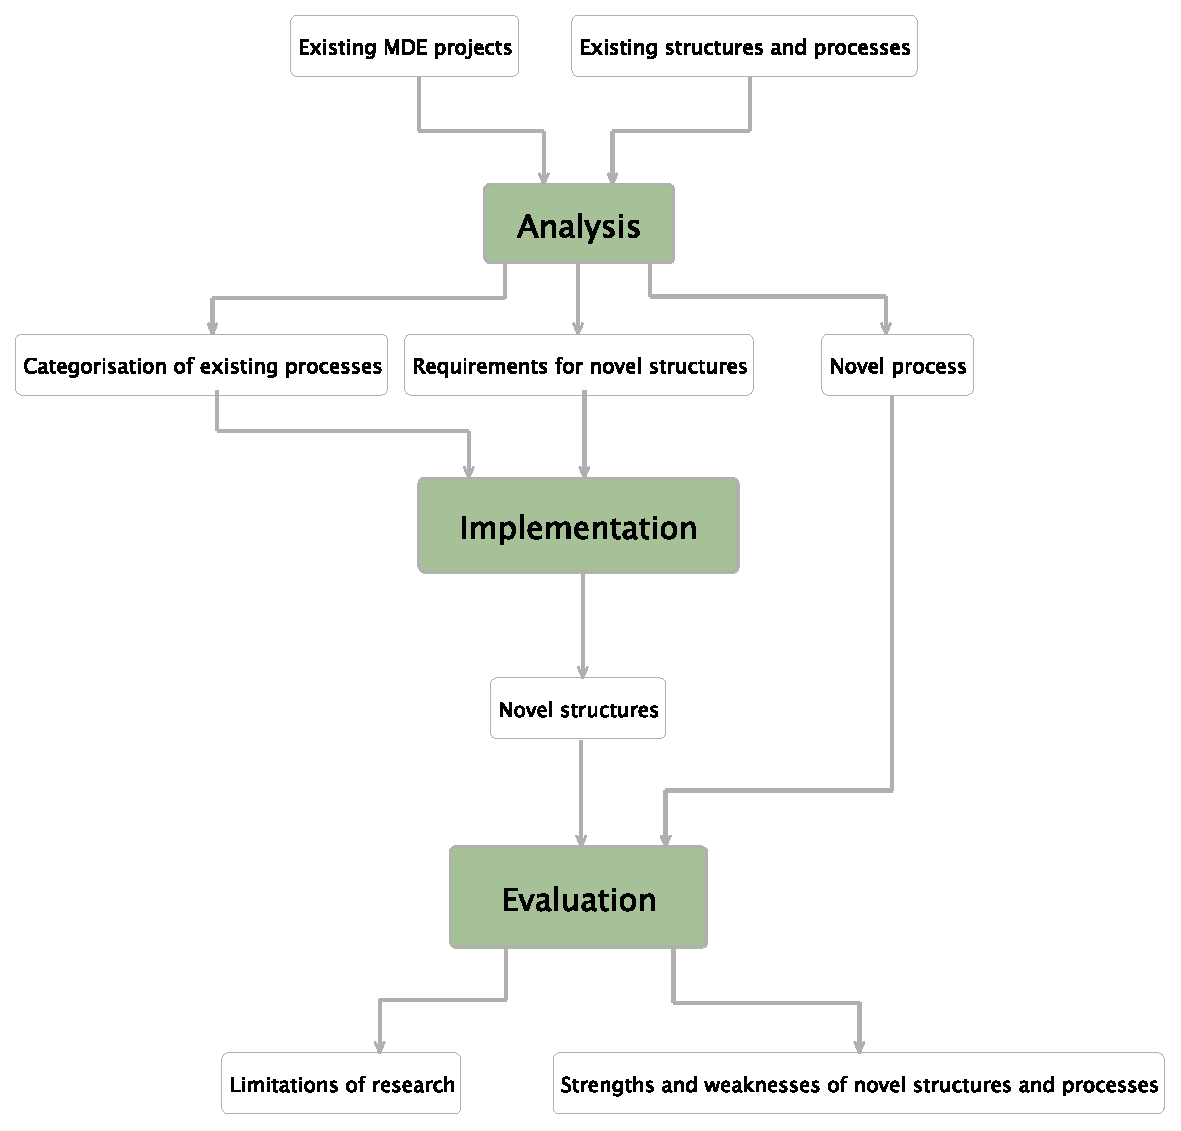
\includegraphics[width=12cm]{1.Introduction/images/method.pdf}
  \end{center}
  \caption{Overview of the research method.}
  \label{fig:research_method}
\end{figure}


Firstly, the \emph{analysis} phase involved studying the evolution of MDE development artefacts in existing projects. The results of the analysis phase were used to determine a category of evolution that lacked support in contemporary MDE development environments, \emph{model-metamodel co-evolution} or, simply \emph{co-evolution}. Co-evolution examples from existing MDE projects were used to categorise existing processes for managing co-evolution, and to formulate requirements for new structures and processes for managing co-evolution. The analysis phase also led to the identification of \emph{user-driven co-evolution}, a process for managing co-evolution that has not previously been recognised in the co-evolution literature.

The \emph{implementation} phase involved proposing, designing and implementing prototypes of novel structures for managing co-evolution, and integrating the prototypical structures with a contemporary MDE environment. The co-evolution examples identified in the analysis phase were used for testing the implementation of the structures.

The \emph{evaluation} phase involved assessing the novel structures for managing co-evolution by comparison to existing structures, and demonstrating the novel process. Evaluation was performed using further examples of co-evolution. To mitigate a possible threat to the validity of the research, the examples used in the evaluation phase were different from those used in the analysis phase. The strengths and weaknesses of the novel and existing structures and processes were synthesised from the comparisons, particularly with respect to the productivity of the development activities that are used to manage co-evolution.

A \cc similar method was successfully used to explore the extent to which component-based applications can be automatically evolved \cite{dig07thesis}. Initially, \cc \emph{analysis} was conducted to identify and categorise evolution in five existing component-based applications, with the hypothesis that many of the changes could be classified as behaviour-preserving \cite{dig06apis}. Examples \cc from the survey facilitated \emph{implementation} of a novel algorithm for the automatic detection of behaviour-preserving changes \cite{dig06detection}. The algorithm was used to implement tools for migrating code in a distributed software development environment \cite{dig06automatic}, and for analysing the history of component-based applications \cite{dig07cms}. The latter facilitated better understanding of program evolution, and refinement of the detection algorithm. Finally, \cc \emph{evaluation} of the tools and detection algorithm was performed by application to three further component-based applications \cite{dig07thesis}.
%!TEX root = /Users/louis/Documents/PhD/Deliverables/Thesis/thesis.tex

\section{Research Results}
\label{sec:research_results}

This thesis proposes novel structures and processes for managing model-metamodel co-evolution. Prototypical reference implementations of the proposed structures have been constructed, including \emph{Epsilon HUTN} (a textual modelling notation) and \emph{Epsilon Flock} (a model migration language). The reference implementations have been constructed atop Epsilon \cite{kolovos09thesis}, an extensible platform for specifying MDE languages and tools, and are interoperable with the Eclipse Modelling Framework \cite{steinberg09emf}, arguably the most widely used MDE modelling framework.

Additionally, this thesis identifies a novel process for managing model-metamodel co-evolution and proposes a theoretical categorisation of existing process for managing model-metamodel co-evolution. The novel process, termed \emph{user-driven co-evolution}, is demonstrated by application to a MDE development process for a real-world project.

The research hypothesis has been validated by comparing the prototypes of the proposed structures and processes with existing structures and processes using examples of evolution from real-world MDE projects. Evaluation has been performed using several approaches, including a collaborative comparison of model migration tools carried out with three MDE experts, comparing quantitive measurements of the proposed and existing migration languages, and application of the proposed structures and processes to two examples of evolution, including an example from a widely used modelling language, the Unified Modelling Language (UML) \cite{uml212}. The evaluation also explored areas in which the prototypical implementations of the proposed structures and processes might be usefully improved to be fit for industrial use.


% Productivity
%  HUTN + MMIS for user-driven co-evolution
%  A choice of user-driven vs developer-driven co-evolution
%  Dedicated migration lang rather than M2M lang for model migration

% Understandability
%  Flock for expressing model migration
%  Use of design patterns / refactorign terminology to describe metamodel evolution
%  HUTN rather than XMI for representating non-conformant models

% Might also mention portability:
%  Migrating between modelling technologies
%  Higher-order migration (migrating between transformation [and other model management?] languages)

%!TEX root = /Users/louis/Documents/PhD/Deliverables/Thesis/thesis.tex

\section{Thesis Structure}
Chapter~\ref{Background} gives an overview of MDE by defining terminology; describing associated engineering principles, practices and tools; and reviewing related areas of computer science. Section~\ref{sec:mde_benefits_and_challenges} synthesises some of the benefits of, and challenges for, contemporary MDE.

Chapter~\ref{LiteratureReview} reviews theoretical and practical software evolution research. Areas of research that underpin software evolution are described, including refactoring, design patterns, and traceability. The review then discusses work that approaches particular categories of evolution problem, such as programming language, schema and grammar evolution. Section~\ref{subsec:mde_evo} surveys work that considers evolution in the context of MDE. Section~\ref{sec:literature_review_summary} identifies three types of evolution that occur in MDE projects and highlights challenges for their management.

Chapter~\ref{Analysis} surveys existing MDE projects and categorises the evolution of MDE development artefacts in those projects. From this survey, the context for the thesis research is narrowed, and the remainder of the thesis focuses on one type of evolution occurring in MDE projects, termed \emph{model-metamodel co-evolution} or simply \emph{co-evolution}. Examples of co-evolution are used to identify the strengths and weaknesses of existing structures and processes for managing co-evolution. From this, Section~\ref{subsec:user-driven_co-evolution} identifies a process for managing co-evolution which has not been recognised previously in the literature, Section~\ref{subsec:co-evolution_categorisation} derives a categorisation of existing processes for managing co-evolution, and Section~\ref{sec:requirements_identification} synthesises requirements for novel structures for managing co-evolution.

Chapter~\ref{Implementation} describes novel structures for managing co-evolution, including a metamodel-independent syntax, which is used to identify, report and to facilitate the reconciliation of problems caused by metamodel evolution. The textual modelling notation described in Section~\ref{sec:notation} and the model migration language described in Section~\ref{sec:flock} are used for reconciliation of models in response to metamodel evolution. The latter provides a means for performing reconciliation in a repeatable manner.

Chapter~\ref{Evaluation} assesses the structures and processes proposed in this thesis by comparison to existing structures and processes. To explore the research hypothesis, several different types of comparison were performed, including an experiment in which quantitive measurements were derived, a collaborative comparison of model migration tools with three MDE experts, and application to a large, independent example of evolution taken from a real-world MDE project.

Chapter~\ref{Conclusion} summarises the achievements of the research, and discusses results in the context of the research hypothesis. Limitations of the thesis research and areas of future work are also outlined.


%!TEX root = /Users/louis/Documents/PhD/Deliverables/ProgressReport/pr.tex
\section{Progress}
Since submitting my qualifying dissertation, I have made progress in four areas. Firstly, I have conducted a thorough review of literature in the areas of co-evolution and synchronisation, enabling elaboration of the aims of my research. Secondly, I have located examples of evolutionary changes occurring during MDE. Thirdly, I have used the examples to evaluate existing techniques for managing evolutionary change in MDE. Fourthly, I have begun to develop a language for specifying evolution. In this section, the progress made in each of these areas is discussed in turn.

In my qualifying dissertation, the term \emph{case study} was used to describe an existing MDE project containing examples of evolution. In this report, the term \emph{example} is preferred.

%!TEX root = /Users/louis/Documents/PhD/Deliverables/ProgressReport/pr.tex
\subsection{Elaboration of Research Aims}
\label{sub:elaboration}
The aim of my research is to develop structures and processes for evolutionary changes in the context of Model-Driven Engineering. Since submitting my qualifying dissertation, I have identified two categories of evolutionary change (for which structures and processes can be developed) by reviewing literature relating to evolution in MDE. Both are discussed below.

\subsubsection{Model and Metamodel Co-Evolution} % (fold)
\label{ssub:model_and_metamodel_co_evolution}
A metamodel is a collection of concepts that are used for specifying models in a particular domain. A model and metamodel are \emph{consistent} when the metamodel specifies every concept used in the model definition. Consistency can be described by a set of constraints between models and metamodels \cite{paige07metamodel}. When all constraints are satisfied, a model and a metamodel are consistent. For example, the Eclipse Modelling Framework\footnote{The Eclipse Modelling Framework (EMF) \cite{steinberg09emf} provides tools for developing, managing and instantiating metamodels.} specifies many constraints for checking model and metamodel consistency: one such constraint is that every object in the model has a corresponding non-abstract class in the metamodel.

A metamodel can evolve (be adapted by a developer), which can cause inconsistency. For example, suppose a concept is removed from a metamodel. Any models that use the removed concept are now inconsistent with the metamodel. \emph{Co-evolution} is the process of evolving both metamodel and model such that they remain consistent. In existing approaches for managing co-evolution (such as \cite{herrmannsdoerfer08cope,cicchetti08automating}), metamodel evolution occurs first, possibly causing models to become inconsistent. Any inconsistent models are then evolved to re-establish consistency.


\subsubsection{Model Synchronisation} % (fold)
\label{ssub:model_synchronisation}
Often, MDE is used to generate code from a model. The MDA guidelines suggest beginning by defining a platform-independent model, and using at least one transformation to produce platform-specific model(s). Code is then generated from the final platform-specific model. When one model evolves, the changes need to be propagated to other models. This activity is termed \textit{model synchronisation}.

Existing model synchronisation literature focuses mostly on enabling \textit{incremental transformation}, a style of model transformation that incrementally updates the target model. For large models, transformation execution time has been shown to be significantly reduced by using incremental transformation \cite{hearnden06incremental}. However, \cite{kolovos08scalability} suggests that building models that are less monolithic (using modularisation) is likely to yield better results than attempting to develop techniques for scaling up model management tasks (such as model transformation). Consequently, I argue that the focus of existing model synchronisation literature is misplaced; model synchronisation research should seek to improve maintainability rather than just simply scalability.  %TODO : read Dimitrios's paper and make this argument strong; "likely to yield better results" is inspecific and weak

Although much of the model synchronisation literature concentrates on incremental transformation, there are other closely-related areas of research, which are more relevant to my work. For instance, \cite{jouault05loosely,drivalos08loosely} describe models of traceability, which could be used to perform \textit{impact analysis} (highlighting the consequences of performing an evolutionary change). Eclipse's Java Development Tools project successfully employs impact analysis for illustrating the effects of Java refactorings \cite{fuhrer07refactoring}. I am unaware of any existing work that explores implementing impact analysis for MDE tools.
%!TEX root = /Users/louis/Documents/PhD/ProgressReport/pr.tex
\subsection{Locating Examples of Evolution}
In my qualifying dissertation, I identified the need for categorising the ways in which MDE development artefacts evolve over time. The categorisation will be used to provide requirements for developing structures and processes for evolutionary changes in the context of model-driven engineering.

A study of example data (existing MDE projects containing evolution) was proposed to produce this categorisation. Work has progressed by defining requirements for candidates for the study. Existing MDE projects were located and analysed against the requirements. Finally, the most suitable candidate projects were selected. As will be discussed in Section \ref{sub:analysis_of_existing_techniques}, the selected projects have been used to analyse existing techniques for managing evolution in MDE.

\subsubsection{Requirements} % (fold)
\label{ssub:requirements}
The requirements defined for candidates for the study of evolution are presented below. In Section \ref{sub:elaboration}, two categories of evolutionary change were identified: model and metamodel co-evolution; and model synchronisation. I wanted to study both. Consequently, requirements were partitioned into three types: those necessary for studying each of the two categories of evolutionary change, and common requirements (applicable to both categories of evolutionary change).

\paragraph{Common requirements}
Every candidate project had to use some aspect of MDE, such as metamodelling or model transformation (requirement R1). In addition, each candidate project had to provide historical information, which elucidated the evolution of development artefacts (R2). For example, several versions of the project from the source code management system. Finally, a candidate project had to contain a sizeable number of significant changes\footnote{`Sizeable' and `significant' are deliberately vague. Further details are given in Section \ref{ssub:project_selection}.} (R3).

\paragraph{Model and metamodel co-evolution}
A candidate project for the study of model and metamodel co-evolution had to define a metamodel and some changes to that metamodel (R4). In the projects considered, the metamodel changes took the form of either (1) another version of the metamodel, or (2) a history (which recorded each of the steps used to produce the adapted metamodel).

A candidate project also had to provide example instances of models before and after each migration activity (R5).

Ideally, a candidate project included more than one consecutive metamodel adaptation, so as to represent the way in which the same development artefacts can continue to evolve over time (optional requirement O1).

\paragraph{Model synchronisation}
A candidate project for the study of model synchronisation had to define a model-to-model transformation (R6).

Furthermore, a candidate project had to include many examples of source and target model for that transformation (R7).

Crucially, a candidate project had to provide many examples of the kinds of change (to either source or target model) that cause inconsistency between the models (R8). 

Ideally, a candidate project also included transformation chains (more than one model-to-model transformation, executed sequentially) (O2). Chains of transformations are prescribed by the MDA guidelines \cite{kleppe03mda}.

% subsubsection requirements (end)

\subsubsection{Project Selection} % (fold)
\label{ssub:project_selection}
Eight candidates were considered for the study. Table \ref{tab:candidates} shows which of the requirements (defined above) are fulfilled by each of the candidates. Each candidate is now discussed in turn.

\begin{table}
	\caption{Candidates for study of evolution in existing MDE projects}
	\centering
	\begin{tabular}{|c||c|c|c||c|c|c||c|c|c|c|}
		\hline
		\multirow{3}{*}{Name} & \multicolumn{10}{|c|}{Requirements} \\
		\cline{2-11}
		          & \multicolumn{3}{|c||}{Common} & \multicolumn{3}{|c||}{Co-evolution} & \multicolumn{4}{|c|}{Synchronisation} \\
		\cline{2-11}
		          & R1 & R2 & R3 & R4 & R5 & O1 & R6 & R7 & R8 & O2 \\
		\hline
		GSN       & x  &    &    & x  &    &    &    &    &    &    \\
		\hline
		Watson    & x  &    &    & x  &    &    & x  &    &    &    \\
		\hline
		Zoos      & x  & x  &    & x  &    &    &    &    &    &    \\
		\hline
		MDT       & x  & x  &    & x  &    & x  &    &    &    &    \\
		\hline
		ModelPlex & x  & x  & x  & x  &    & x  & x  & x  &    &    \\
		\hline
		FPTC      & x  & x  & x  & x  & x  &    &    &    &    &    \\
		\hline
		xText     & x  & x  & x  & x  & x  & x  & x  & x  &    & x  \\
		\hline
		GMF       & x  & x  & x  & x  & x  & x  & x  & x  &    & x  \\
		\hline
	\end{tabular}
	\label{tab:candidates}
\end{table}

\paragraph{GSN} % (fold)
\label{par:gsn}
Georgios Despotou and Tim Kelly are constructing a metamodel for Goal Structuring Notation (GSN). The metamodel has been developed incrementally. There is no accurate and detailed version history for the GSN metamodel (requirement R2). \textbf{Suitability for study:} Unsuitable.
% paragraph gsn (end)

\paragraph{OMG} % (fold)
\label{par:omg}
Andrew Watson references the development of two MDE projects in \cite{watson08mdahistory}. I emailed Watson to ascertain whether the source code for the studies was available. Source code was available for one of the projects, but there is no version history. \textbf{Suitability for study:} Unsuitable.
% paragraph omg (end)

\paragraph{Zoos} % (fold)
\label{par:zoos}
There are several collections of popular metamodels available in \emph{zoos}. Each zoo contains metamodels authored in one metamodelling language (e.g. EMF's Ecore). I considered two zoos for this study, but neither contained any significant metamodel changes. Those changes that were made involved only renaming of meta-classes (trivial to migrate) or additive changes (which do not affect consistency, and therefore require no migration). \textbf{Suitability for study:} Unsuitable.
% paragraph zoos (end)

\paragraph{MDT} % (fold)
\label{par:mdt}
The Eclipse Model Development Tools (MDT) \cite{mdt} provides implementations of industry-standard metamodels, such as UML2 \cite{uml212} and OCL \cite{ocl2}. Like the metamodel zoos, the version history for the MDT metamodels contained no significant changes. \textbf{Suitability for study:} Unsuitable.
% paragraph mdt (end)

\paragraph{ModelPlex} % (fold)
\label{par:modelplex}
Jendrik Johannes has made available to me work from the European project, ModelPlex. Johannes's work involves transforming UML models to Tool Independent Performance Models (TIPM) for simulation. Although the TIPM metamodel and the UML-to-TIPM transformation have been changed significantly, no significant changes have been made to the models. \textbf{Suitability for study:} Unsuitable.
% paragraph modelplex (end)

\paragraph{FPTC} % (fold)
\label{par:fptc}
Failure Propagation and Transformation Calculus (FPTC) provides a means for reasoning about the failure behaviour of complex systems. Before starting my doctorate, I worked with Richard Paige to develop an implementation of FPTC in Eclipse. The implementation includes an FPTC metamodel. Recent work with Philippa Conmy identified a significant flaw in the implementation, leading to changes to the metamodel. These changes caused existing FPTC models to become inconsistent with the metamodel. Conmy has made available to me copies of FPTC models from before and after the changes. \textbf{Suitability for study:} Suitable for model and metamodel co-evolution. Unsuitable for studying model synchronisation.
% paragraph fptc (end)

\paragraph{xText} % (fold)
\label{par:xtext}
xText is an openArchitectureWare (oAW) \cite{oaw} tool for generating parsers, metamodels and editors for performing text-to-model transformation. Internally, xText defines a metamodel, which has been changed significantly over the last year. In several cases, changes have caused inconsistency with existing models (such as the ones used in the FPTC project). xText provides examples of use, which have been updated alongside the metamodel. \textbf{Suitability for study:} Suitable for studying model and metamodel co-evolution. Unsuitable for studying model synchronisation.
% paragraph xtext (end)

\paragraph{GMF} % (fold)
\label{par:gmf}
The Graphical Modelling Framework (GMF) \cite{gronback06gmf} allows the definition of graphical concrete syntax for metamodels that have been defined in EMF. GMF prescribes a model-driven approach: Users of GMF define concrete syntax as a model, which is used to generate a graphical editor. In fact, five models are used together to define a single editor using GMF.

GMF defines the metamodels for graphical, tooling and mapping definition models; and for generator models. The metamodels have changed considerably during the development of GMF. Some changes have caused inconsistency with GMF models. Presently, migration is encoded in Java. Gronback\footnote{Private communication, 2008.} has stated that the migration code is being ported to QVT (a model-to-model transformation language) as the Java code is difficult to maintain.

GMF fulfils almost all of the requirements for the study. A large amount of data for the co-evolution of metamodels and models is available, including migration strategies. The GMF source code repository does not contain examples of the kinds of change that cause inconsistency between the models. However, GMF has a large number of users, and it may be possible to gather this information elsewhere. \textbf{Suitability for study:} Suitable for studying both categories of evolutionary change.
% paragraph gmf (end)

\paragraph{Summary of selection}
The FPTC and xText projects were selected for a study of model and metamodel co-evolution. No appropriate projects were located for a study of model synchronisation. The GMF project will not be studied now, but reserved as a case study for evaluating my research.

\subsubsection{Other data} % (fold)
\label{ssub:other_data}
As only a small number of candidate projects fulfilled all of the requirements, I decided to collect additional data from alternative sources. Firstly, I sought examples from related domains (e.g. object-oriented systems) for suitable data. Secondly, I am collaborating with colleagues from two projects, both of which are using iterative and incremental model-driven development. Example data for both categories of evolutionary change will be available from these two projects.

\paragraph{Examples of evolution from object-oriented systems} % (fold)
\label{par:examples_of_evolution_from_object_oriented_systems}
In object-oriented programming, software is constructed by developing groups of related objects. Every object is an instance of (at least) one class. A class is a description of characteristics, which are shared by each of the class's instances (objects).

A similar relationship exists between models and metamodels: metamodels comprises meta-classes, which describe the characteristics shared by each of the meta-class's instances (elements of a model). Together, model elements are used to describe one perspective (model) of a system

Consequently, I believe that studying the evolution of object-oriented systems will yield results that are relevant to the model and metamodel co-evolution occurring in MDE. To support this argument, I have performed a preliminary study of frequently observed changes made to object-oriented systems.

\subparagraph{Preliminary study of object-oriented refactorings} % (fold)
\label{subp:preliminary_study_of_object_oriented_refactorings}
\emph{Refactoring} is the process of improving the structure of existing code while maintaining its external behaviour. When used as a noun, a refactoring is one such improvement. \cite{fowler99refactoring} provides a catalogue of refactorings for object-oriented systems. For each refactoring, Fowler gives advice and instructions for its application.

Fowler's refactorings provide examples of evolutionary changes to object-oriented systems. I attempted to apply each of Fowler's refactorings to EMF metamodels and discovered that some are irrelevant to metamodelling. Those refactorings that do not apply to EMF metamodels belong to one of three categories:

\begin{enumerate}
	\item \textbf{Operational refactorings} focus on restructuring behaviour (method bodies). EMF does not support the specification of behaviour in models.
	\item \textbf{Navigational refactorings} convert, for example, between bi-directional and uni-directional associations. These changes are non-breaking in EMF, which automatically provides values for the inverse of a reference when required.
	\item \textbf{Domain-specific refactorings} manage issues specific to object-oriented programming, such as casting, defensive return values, and assertions. These issues are not relevant to metamodelling.
\end{enumerate}

The object-oriented refactorings that can be applied to metamodels provide examples of metamodel evolution. When applied, some of these refactorings potentially cause inconsistency between a metamodel and its models. I used Fowler's description of each refactoring to deduce a migration strategy for updating (co-evolving) inconsistent models. An example of deducing a migration strategy is now presented.

Figure \ref{fig:refactoring} illustrates a refactoring that changes a reference object to a value object. Value objects are immutable, and cannot be shared (i.e. any two objects cannot refer to the same value object). Reference objects are mutable, and can be shared. Figure \ref{fig:refactoring} indicates that applying the refactoring restricts the multiplicity of the association (on the Order end) to 1 (implied by the composition); prior to the refactoring the multiplicity is many.

\begin{figure}[htbp]
  \begin{center}
    \leavevmode
    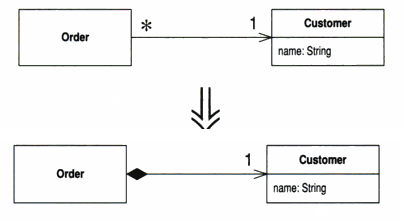
\includegraphics[scale=0.5]{refactoring.png}
  \end{center}
  \caption{Refactoring a reference to a value. Taken from \cite{fowler99refactoring}[pg183]}
  \label{fig:refactoring}
\end{figure}

Before applying the refactoring, each customer may be associated with more than one order. After the refactoring, each customer should be associated with only one order. Fowler indicates that every customer associated with more than one order should be duplicated, such that one customer object exists for each order. Therefore, the migration strategy in Listing \ref{lst:refactoring} is deduced.

\begin{lstlisting}[caption=Migration strategy for the refactoring in pseudo code., label=lst:refactoring]
for every customer, c
	for every order, o, associated with c
		create a new customer, d
		copy the values of c's attributes into d
	next o
	
	delete c
next c
\end{lstlisting}

Using this process, I deduced migration strategies for each of the refactorings that were (1) applicable to EMF metamodels, and (2) caused inconsistencies between a metamodel and its models. Since, I have recognised some of the metamodel changes in the FPTC project (one of the projects chosen for the model and metamodel co-evolution study) as object-oriented refactorings.

Object-oriented refactorings are used to improve the maintainability of existing systems. In other words, they represent only one of the three reasons for evolutionary change defined by \cite{sjoberg93quantifying}. The two other types of changes to object-oriented systems are equally relevant to my research. Consequently, I have obtained further examples of changes made to object-oriented systems from Tim Hoverd, an experienced object-oriented developer. Hoverd's examples include changes made that represent at least one of the other reasons for evolutionary change defined by \cite{sjoberg93quantifying}.

% subparagraph preliminary_study_of_object_oriented_refactorings (end)
% paragraph examples_of_evolution_from_object_oriented_systems (end)


\paragraph{Collaborations} % (fold)
\label{par:collaborations}
As well as locating example data from object-oriented programs, I am currently collaborating with two colleagues who are using MDE. Adam Sampson and I are constructing a metamodel to standardise the way in which his team model process-oriented programs. Heather Barber and I are investigating the feasibility of implementing a tool for generating story-worlds for interactive narratives.

In both cases, the work will involve constructing a metamodel for describing concepts in the domain. The metamodels will be developed incrementally, and consequently will change over time. In both cases, the domain is large, so I am hopeful that evolution will involve more than just additive changes. If so, the data will be used for studying model and metamodel co-evolution.

Both parties have expressed an interest in transforming their models to generate code (possibly via an intermediate model). If realised, the data will be used for studying model synchronisation.

% paragraph collaborations (end)
% subsubsection other_data (end)

\subsubsection{Summary}
To summarise, I have located eight existing MDE projects, three of which contain data that can be analysed to obtain requirements for the development of structures and process for evolutionary changes in the context of model and metamodel co-evolution occurring during model-driven engineering. One of the three projects, GMF, will be reserved as a case study for my thesis. Refactorings and other examples from object-oriented programming will supplement the data available from the existing MDE projects. Collaboration with Sampson and Barber will yield further data.

As I have been able to locate more examples of model and metamodel co-evolution than model synchronisation, I have decided to proceed by focusing on developing structures and processes for model and metamodel co-evolution. Should I discover further sources of model synchronisation, I will expand my research accordingly.





%!TEX root = /Users/louis/Documents/PhD/ProgressReport/pr.tex
\subsection{Analysis of Existing Techniques}
\label{sub:analysis_of_existing_techniques}


\subsubsection{Model and Metamodel Co-Evolution}
    Analysed the most promising tools using data from a real-world system.

    Presented HUTN at MoDELs. At the same conference, a tool (called COPE) for managing model and metamodel co-evolution was presented. COPE makes use of a generic syntax for performing model migration and metamodel evolution.



		\subsection{Development}
		\label{ssec:development}
		    Begun cataloguing types of model evolution. Started with Fowler's refactorings, and now expanding to incorporate evolutions seen in real-world systems.


%!TEX root = /Users/louis/Documents/PhD/Deliverables/ProgressReport/pr.tex
\section{Plan}
I have completed several of the activities outlined in the plan that was presented in my qualifying dissertation. However, I have experienced some difficulties when following that plan. A revised plan is presented in Section \ref{sub:revised_plan}. A discussion of the main goals of my research activities, and their relationship to the revised plan, is presented in Section \ref{sub:goals}.


\subsection{Existing Plan}
\label{sub:existing_plan}
Figure \ref{fig:old_plan} shows the research plan presented in my qualifying dissertation. I identified four activities to be completed before submitting my progress report. The status of those activities is as follows:

\begin{itemize}
	\item \textbf{Locate case studies}: Completed, as discussed in Section \ref{sub:examples}. However, locating example data took longer than I estimated in Figure \ref{fig:old_plan}. This caused ``Analyse case studies'' to start later than planned.
	\item \textbf{Analyse case studies}: Somewhat completed, as discussed in Section \ref{sub:analysis_of_existing_techniques}. In summary, I still need to use the example data to complete a review of existing co-evolution tools.
	\item \textbf{Co-evo and runtime evo lit review}: Completed, although I decided to focus more on model synchronisation literature, than runtime evolution literature as I found the former more interesting. The literature review lead to the elaboration of research aims discussed in Section \ref{sub:elaboration}.
	\item \textbf{Write progress report}: Completed.
\end{itemize}

In addition, I have made progress with the ``Plan metamodel evolution language'' activity, as discussed in Section~\ref{sub:development}. Although work on this activity was not due to start until February 2009, I proceeded while waiting for responses to requests for data for the ``Locate case studies'' activity.


\subsection{Revised Plan}
\label{sub:revised_plan}
Figure \ref{fig:revised_plan} shows my revised research plan. Originally, I had intended to begin planning a language for performing co-evolution in February 2009. However, I now feel that I am not yet able to identify requirements for the language. Consequently, I have introduced several new activities (``Plan stakeholder survey'', ``Analyse COPE'', ``Analyse Cicchetti's work'', ``Collaborate with Barber'', ``Collaborate with Sampson'') that will aid in defining requirements. These new activities are discussed in Section \ref{sub:goals}. Hence, the activities relating to developing the metamodel evolution language have been delayed. Furthermore, ``Develop metamodel evolution language'' and ``Evaluate user feedback'' now occupy one month (rather than six weeks) as I have already made some progress as discussed in Section \ref{sub:development}. Finally, Q4 2009 has also been updated to better reflect the progress made during that period.

% TODO: Evaluate user feedback seems unreasonable. Where will the feedback be obtained from?

When trying to follow the plan in Figure \ref{fig:old_plan}, I encountered some further difficulties. Firstly, some of the activities were too broad (such as ``Analyse case studies'' and ``Co-evo and runtime evo lit review'') and I had not identified clear goals, making progress hard to measure. Secondly, activities were unrealistically scheduled over the Christmas period.  In my revised plan (Figure \ref{fig:revised_plan}), I have decomposed large activities into several smaller activities. Goals for each of the activities are outlined in Section \ref{sub:goals}. In addition, I have not scheduled any activities during Christmas and Easter vacations.

\clearpage
\setlength\paperheight{297mm}
\setlength\paperwidth{420mm}
\setlength\pdfpageheight{\paperheight}
\setlength\pdfpagewidth{\paperwidth}

\includepdf[scale=1, pages={1-2}, addtolist={1,figure,{foo},fig:old_plan,2,figure,{foo},fig:revised_plan}]{plan_figures.pdf}

\setlength\paperheight{297mm}
\setlength\paperwidth{210mm}
\setlength\pdfpageheight{\paperheight}
\setlength\pdfpagewidth{\paperwidth}

\subsection{Goals} % (fold)
\label{sub:goals}
Over the next three months, my primary goal is to determine requirements for a co-evolution language. The requirements will be identified by using examples of evolution from existing MDE projects to analyse existing co-evolution tools, by collaborating on incremental metamodel development with Barber and with Sampson, and by performing a survey of developers working on existing MDE projects.

Over the next year, I will use these requirements to develop structures and processes for co-evolutionary changes in the context of model-driven engineering. Specifically, I will develop a language for describing and executing co-evolution. Best practices for using the language will be identified by application to examples of evolution in existing MDE projects.

I anticipate that further structures and processes will be required to fulfil all of the identified requirements. Therefore, I will also develop an algorithm for automatically inferring migration strategies in response to metamodel changes.

My research will be evaluated using the Graphical Modelling Framework (GMF) \cite{gronback06gmf} as a case study. I will demonstrate that those problems occurring in GMF caused by evolutionary change can be managed using the structures and processes that I develop.

\subsubsection{February to June 2009}
I have identified several activities to be completed before I submit my thesis outline at the end of June 2009. Goals for each of these activities are now described. My thesis outline will contain goals for the activities to be performed between July 2009 and December 2009.

\paragraph{Plan stake-holder survey} % (fold)
\label{par:plan_stakeholder_survey}
No existing co-evolution research identifies requirements from developers working on MDE projects. By surveying developers working on existing MDE projects, I will ascertain data which will be used to derive requirements for my research. The survey will find answers to the following types of questions: Which tools are developers using for editing and versioning their models and metamodels? Are developers regularly introducing inconsistencies between their models and metamodels? Are developers performing co-evolution manually or using a tool? Which tools are being used for co-evolution?

I will survey developers working on MDE projects. I will seek participants from MODELPLEX, a European project focusing on using MDE to perform complex systems modelling, and conferences that discuss evolution in MDE (such as MCCM 2009). 

Before devising the survey, I will speak to members of the York Human Computer Interaction group, such as Chris Power and Paul Cairns. Both Power and Cairns have experience in developing surveys.

\subparagraph{Goals:} Devise and conduct a survey of developers working on existing MDE projects. Identify a process for devising an effective survey. Determine suitable questions, and use the answers to derive requirements for my thesis.

% paragraph plan_stakeholder_survey (end)


\paragraph{Analyse COPE and Cicchetti's work} % (fold)
\label{par:analyse_existing_work}
As discussed in Section \ref{sub:analysis_of_existing_techniques}, \cite{herrmannsdoerfer08cope,cicchetti08automating} both describe tools for performing co-evolution. By analysing both tools with data located from existing MDE projects, I will continue to identify areas in which these tools are effective, and ways in which they may be improved. The analysis will provide requirements for my research.

\subparagraph{Goals:} Use the example data discussed in Section \ref{sub:examples} to determine the effectiveness and shortcomings of existing tools for performing automated co-evolution. Use the findings to derive requirements for my research.

% paragraph analyse_existing_work (end)


\paragraph{Collaborate with Barber and with Sampson} % (fold)
\label{par:collaborate_with_barber_and_with_sampson}
I will continue to collaborate with Barber and with Sampson to iteratively and incrementally produce metamodels as discussed in Section \ref{par:collaborations}. Initially, I will collect a record of evolutionary changes made during the development of metamodels. If we encounter any evolutionary changes that inhibit development, I will be able to derive further requirements for my research.

\subparagraph{Goals:} Determine the extent to which the development of Barber's and Sampson's metamodels will aid my research. Observe and record any evolutionary changes made during the development. Obtain requirements from the data, and from Barber's and Sampson's experiences with MDE.

% paragraph collaborate_with_barber_and_with_sampson (end)


\paragraph{Plan metamodel evolution language} % (fold)
\label{par:plan_metamodel_evolution_language}
Before beginning any development, I will consolidate the results of previous activities to produce requirements for a co-evolution language. In addition, I will begin to prototype the language. The primary aim of the prototype will be for me to gain experience with any unfamiliar technologies.

\subparagraph{Goals:} Produce a list of requirements for a co-evolution language. Investigate any unfamiliar technologies that may aid in the development of the language.

% paragraph plan_metamodel_evolution_language (end)


\paragraph{Write paper for MoDELS / SLE / MCCM 2009} % (fold)
\label{par:write_paper_for_models_sle_mccm_2009}
The research conducted before July 2009 will yield publishable results. In particular, the collaboration with Barber will be used to generate a report describing our experiences with current MDE tools. We will be able to highlight the need for automated co-evolution tools and discuss why this need is not yet being fulfilled. The paper will strengthen the case for a claim that I will make in my thesis: that structures and processes for managing co-evolution are required in the context of model-driven engineering, and that existing tools are not satisfying this requirement.

\subparagraph{Goals:} Publish a paper at MoDELS 2009 (or co-located conferences). The paper will provide a basis for a chapter of my thesis.
% paragraph write_paper_for_models_sle_mccm_2009 (end)


\subsection{Summary}
In this report, software evolution and its impact on the maintainability of systems engineering using model-driven techniques have been introduced. Chapter \ref{sec:progress} restated and elaborated the aims of my research, presented the MDE projects that I will use to explore the effects of evolutionary change, discussed my analysis of existing tools for performing automated co-evolution; and presented the development status of a language for specifying and executing co-evolution.

Throughout this chapter, goals for developing my research have been presented, along with a timetable. The primary aim of my research will to be to produce requirements for, implement, and evaluate a language for specifying and executing co-evolution in the context of model-driven engineering.

\bibliography{pr}
\bibliographystyle{longname}

\end{document}
